\chapter{Trustable Oracles }\label{chap:chap3}

\section*{}
%Este capítulo deve começar por fazer uma apresentação detalhada do
%problema a resolver\footnote{Na introdução a apresentação do
%  problema foi breve.} podendo mesmo, caso se justifique,
%constituir-se um capítulo com essa finalidade.

%Deve depois dedicar-se à apresentação da solução sem detalhes de
%implementação. 
%Dependendo do trabalho, pode ser uma descrição mais teórica, mais
%``arquitetural'', etc.





\section{Defining Trust}

At this point, a definition of what trust in a oracle is seems appropriate. Trust has a lot of meanings, depending on the needs of all the parties involved. I will model several levels of trust and the requirements and fallacies of each model as well as its application and drawbacks.

Starting from an absolute trust scenario, in this model, the end user, being the smart contract which receives information provided by the oracle, has complete assurances from both the veracity of the data provided by the data-source, as well as, undeniable proof that the oracle did not tamper with the relayed information. This scenario points out two main points of failure, either maliciously or unintentionally. 

The first component which can be faulty or compromised is the data-source. Assuring that the information provided is correct does not have a straightforward answer. What correct means is open to interpretation. For example, if the data source is an IoT sensor, which is prone to failures, being correct is relative. The sensor needs to be perfectly calibrated and accurate. In this case, using several sensors and averaging its values or removing outliers would solve its correctness. Another example, could be an API that returns the current value of the EUR in USD. In this scenario a party that would benefit from a higher conversion than the real one could coerce or attack the data-source into providing a favorable value. The answer here can also be using several data-sources. Another solution would be to use a highly trusted entity such as the European Central Bank (ECB) which can be a lot harder to coerce or attack and having a signatures from the ECB that backs the provided data. Choosing what type of data-source to use has a huge impact on the trust fullness of the provided data not to mention architecture centralization when using a source such as the ECB. All in all, the end user will have to understand the requirements and level of trust necessary.

The second, and most relevant for analysis, is the oracle service used. Oracles are a necessary part of the process, since the other option would be having the data providers adapting to the blockchain which does not seem to be a realistic option at the moment. Therefore we most trust an oracle or a group of oracles. Two main options are available, either trusting a third-party oracle or self deploying an oracle. In the first scenario, three variables take part in the level of trust. Firstly he third-party oracle, if paid for, has the monetary incentive to be honest, since a bad record of dishonesty would have the service loosing credibility and therefore clients. Secondly, by using proofs the oracle can establish its legitimacy, as long as, the proofs can undoubtedly be trusted and verifiable by the smart contract, I will later analyse in depth this issue. Finally, oracle execution transparency by using open-source code and having means for being audit. Additionally to guaranteeing single oracle integrity, it may be in the interest of the user to use several oracles either to provide service availability or to increase trust by combining the result from different oracle services. 


\section{Oracle Architectures}


\begin{figure*}[t]
  \begin{center}
    \leavevmode
    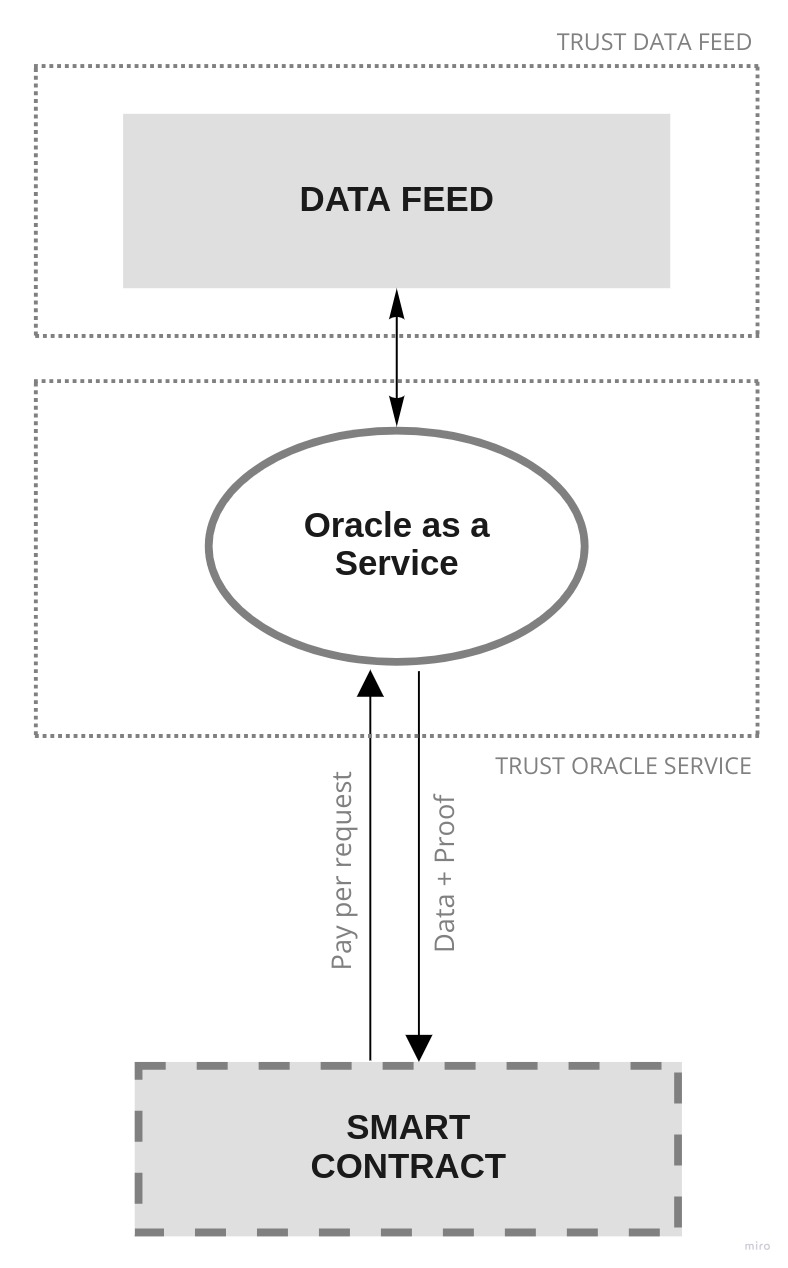
\includegraphics[width=0.5\textwidth]{figures/oraclearch1.jpg}
    \caption{Oracle as a Service w/ Single Data Feed.}
    \label{fig:/figures/paper-screening}
  \end{center}
\end{figure*}

\begin{figure*}[t]
  \begin{center}
    \leavevmode
    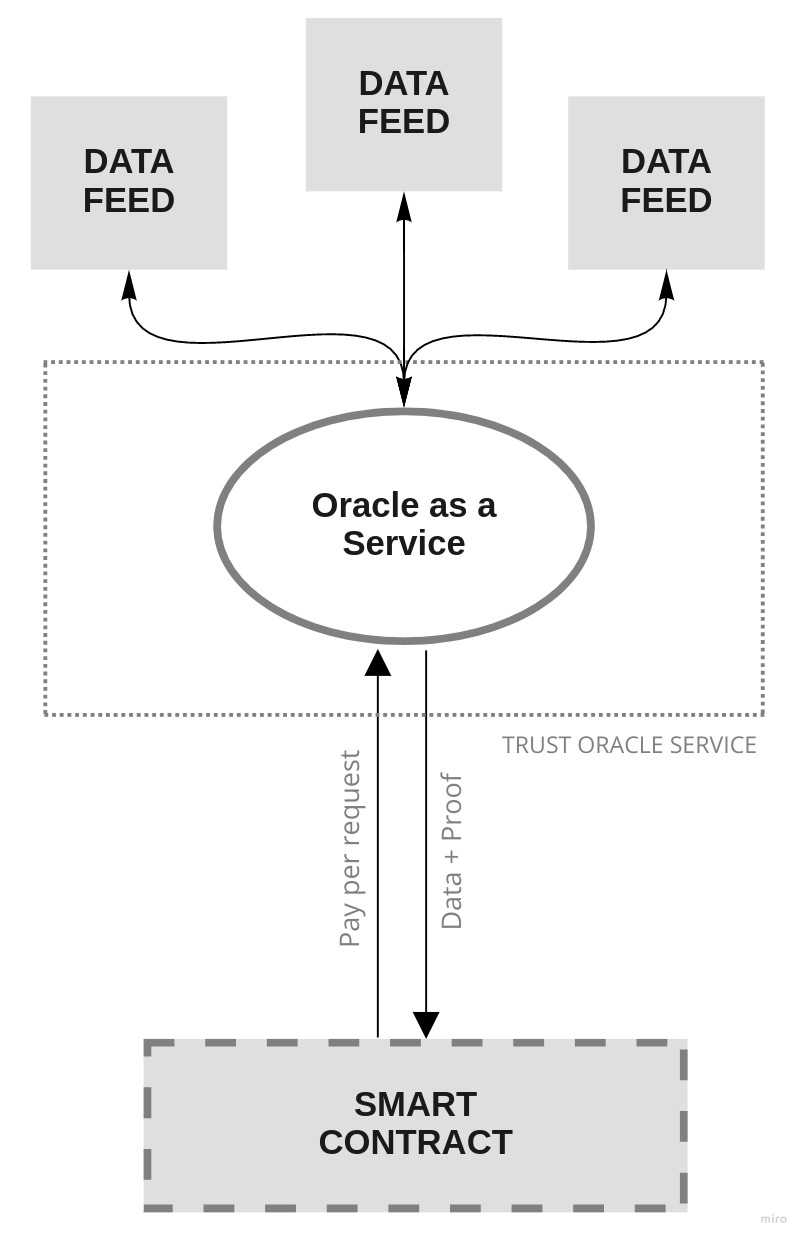
\includegraphics[width=0.5\textwidth]{figures/oraclearch2.jpg}
    \caption{Oracle as a Service w/ Multiple Data Feeds.}
    \label{fig:/figures/paper-screening}
  \end{center}
\end{figure*}

\begin{figure*}[t]
  \begin{center}
    \leavevmode
    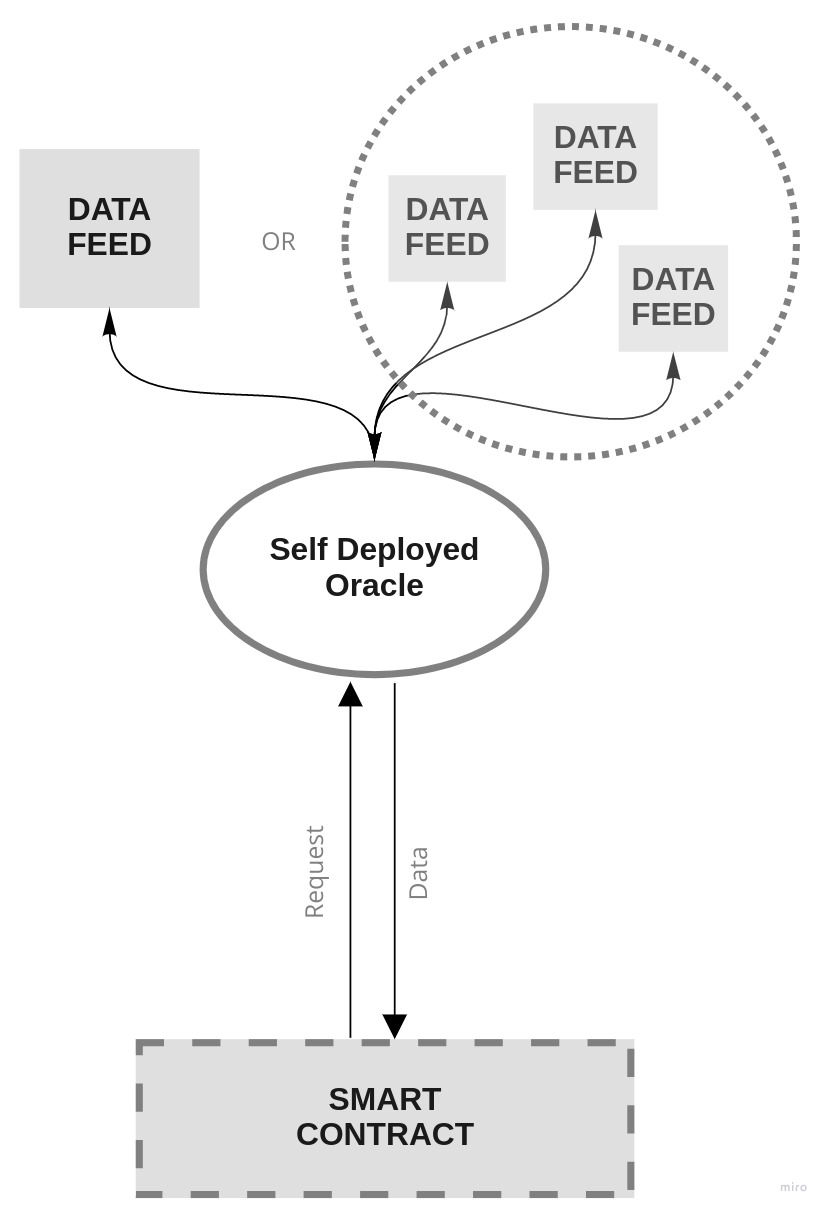
\includegraphics[width=0.5\textwidth]{figures/oraclearch3.jpg}
    \caption{Single-Party Self Hosted Oracle.}
    \label{fig:/figures/paper-screening}
  \end{center}
\end{figure*}

\begin{figure*}[t]
  \begin{center}
    \leavevmode
    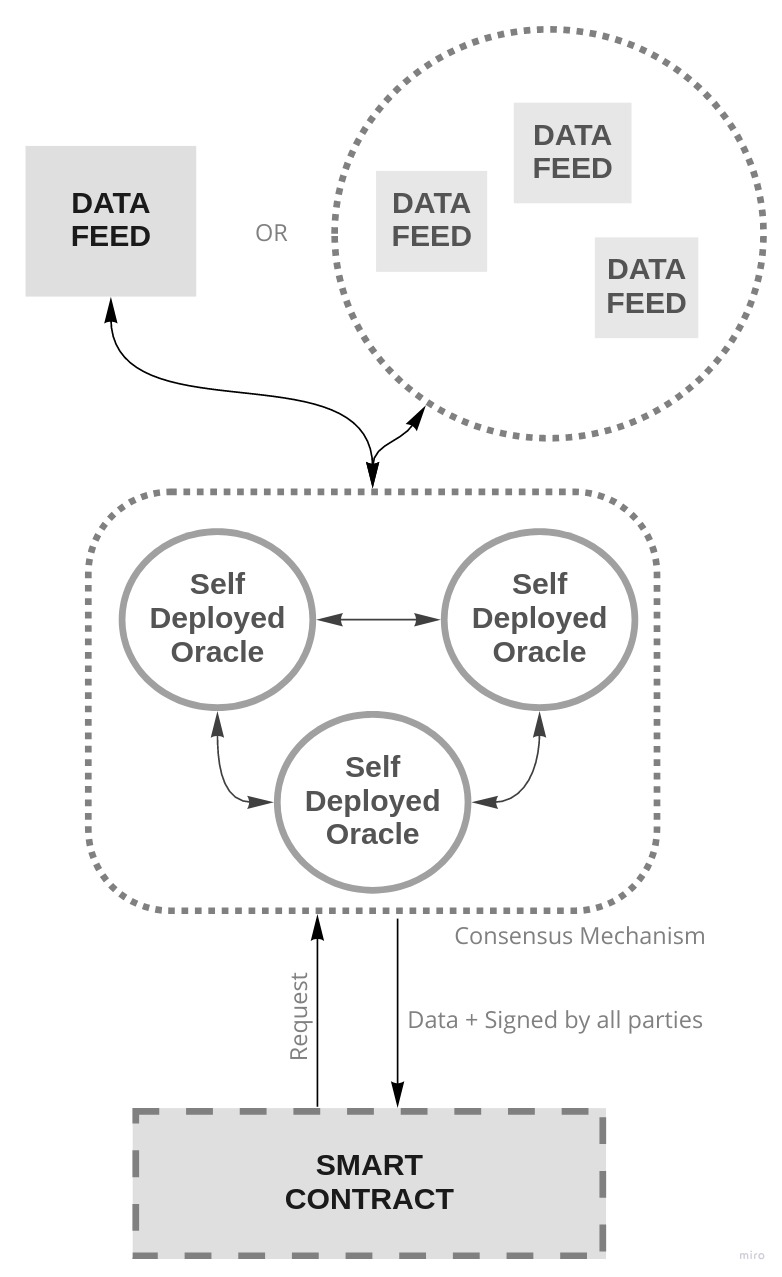
\includegraphics[width=0.5\textwidth]{figures/oraclearch4.jpg}
    \caption{Multi-Party Self Hosted Oracle.}
    \label{fig:/figures/paper-screening}
  \end{center}
\end{figure*}


\section{Summary and conclusions}
